% IEEE-style journal paper for the sb-video-interpolation repo
% Compile: pdflatex -> bibtex -> pdflatex -> pdflatex
\documentclass[journal]{IEEEtran}

\usepackage{amsmath,amssymb}
\usepackage{graphicx}
\usepackage{cite}
\usepackage{booktabs}
\usepackage{array}
\usepackage{url}
\usepackage[hidelinks]{hyperref}

% Optional: improves line breaks for long equations
\allowdisplaybreaks

\title{Soft-Constrained Schr\"{o}dinger Bridge Video Editing in Stable Diffusion Latent Space}

\author{
\IEEEauthorblockN{
\begin{minipage}{.3\textwidth}
        \centering
        Nivya Muchikel\\
        \textit{Department of Mathematics} \\
        \textit{RV College of Engineering}\\
        Bengaluru, India \\
    \end{minipage}
    \hspace{.03\textwidth}
    \begin{minipage}{.3\textwidth}
        \centering
        Sharanya Madhyastha\\
        \textit{Department of Computer Science} \\
        \textit{RV College of Engineering}\\
        Bengaluru, India \\
    \end{minipage}
    \hspace{.03\textwidth}
    \begin{minipage}{.3\textwidth}
        \centering
        Srikar Rao H M\\
        \textit{Department of Computer Science} \\
        \textit{RV College of Engineering}\\
        Bengaluru, India \\
    \end{minipage}
    }
    }



\begin{document}
\maketitle

\begin{abstract}
Diffusion-based generative models provide strong semantic controllability but often fail to preserve temporal coherence and physical structure when editing existing videos. We present a text-guided video editing framework based on a soft-constrained Schr\"{o}dinger Bridge (SB) formulation operating in the latent space of a pretrained Stable Diffusion variational autoencoder (VAE). Video frames are treated as particles transported through a learned time-conditioned drift field between a source latent trajectory and a stochastic target distribution. The drift field is predicted by a lightweight \emph{DriftNet} built by freezing a pretrained Stable Diffusion 2D U-Net for per-frame spatial priors and training only a small 3D temporal residual module for frame-to-frame consistency. Semantic alignment is incorporated via CLIP text embeddings and a penalty-based terminal constraint, while temporal consistency is encouraged by a bridge-matching objective. Sampling is performed by a backward Euler--Maruyama solver in latent space followed by VAE decoding to reconstruct edited video frames.
\end{abstract}

\begin{IEEEkeywords}
Schr\"{o}dinger bridge, diffusion models, video editing, latent diffusion, CLIP guidance, temporal consistency, stochastic differential equations.
\end{IEEEkeywords}

\section{Introduction}
Video editing systems aim to improve creative expression, content accessibility, and visual storytelling. However, many current generative editing pipelines suffer from (i) lack of temporal coherence (e.g., flicker), (ii) vulnerability to semantic drift during generation, and (iii) limited accessibility for non-technical users who cannot author complex prompts or scripts. Diffusion-based generative models have demonstrated powerful image synthesis and editing capabilities, yet na\"{\i}vely applying per-frame diffusion to video can disrupt physical structure and motion, yielding temporally inconsistent results.

This work proposes a text-guided video editing framework using \emph{soft-constrained Schr\"{o}dinger bridges}. We view a video as a sequence of latent variables transported through a learned vector field from a source distribution toward a target distribution. A U-Net neural network model with attention-based conditioning is used to estimate the velocity of this flow~\cite{ronneberger2015unet,vaswani2017attention}. The model is guided by two objectives: a bridge matching loss that promotes temporal coherence and a CLIP-based soft constraint that aligns edits with the text prompt semantics. To reduce computational cost while preserving high-level content, the system operates in the latent space of a pretrained VAE (Stable Diffusion). Sampling uses an Euler--Maruyama stochastic differential equation (SDE) solver.

\subsection{Contributions}
This paper (and accompanying repository) makes the following contributions:
\begin{itemize}
\item A soft-constrained Schr\"{o}dinger bridge formulation for text-guided video-to-video editing in latent space.
\item An implementation that reuses a Stable Diffusion 2D U-Net for per-frame spatial priors and trains only a small 3D temporal residual for consistency.
\item Practical engineering details for caching VAE latents and text embeddings to enable efficient experimentation.
\item A reproducible reference pipeline for training and inference using backward Euler--Maruyama integration in latent space.
\end{itemize}

\section{Related Work}
We position our approach among recent directions in Schr{\"{o}}dinger bridges, optimal transport, diffusion/latent diffusion modeling, and text-guided video editing.

\subsection{Schr\"{o}dinger Bridges and Optimal Transport}
Schr\"{o}dinger bridge (SB) problems connect entropic optimal transport with controlled stochastic processes and can be interpreted as finding the most likely stochastic dynamics consistent with marginal constraints while remaining close to a reference diffusion in relative entropy. Modern SB literature emphasizes (i) control-theoretic reformulations, (ii) efficient solvers in high-dimensional state spaces, and (iii) learning-based approximations that replace iterative procedures with neural drift parameterizations.

Classical surveys connect the Schr\"{o}dinger problem to entropy-regularized optimal transport and stochastic control~\cite{leonard2014survey}. Entropic optimal transport is also computationally attractive because Sinkhorn-style regularization yields scalable solvers~\cite{cuturi2013sinkhorn}. In generative modeling, diffusion Schr\"{o}dinger bridges reinterpret score-based sampling as finite-time transport between data and prior distributions~\cite{debortoli2021dsb}. Generalized and augmented bridge matching objectives broaden the class of corruption paths and targets that can be matched with neural drifts~\cite{liu2023generalized,debortoli2023augmented}. Soft-constrained SB formulations relax terminal constraints with penalties to trade off strict adherence to a target against fidelity to the reference process~\cite{garg2024softconstrained}.

\subsection{Diffusion and Latent Diffusion Models}
Denoising diffusion models build on nonequilibrium thermodynamic views of iterative corruption and reversal~\cite{sohldickstein2015deep}. Denoising diffusion probabilistic models (DDPMs) model data generation as iterative denoising from Gaussian noise with time-conditioned neural networks~\cite{ho2020ddpm}, while score-based SDE formulations describe generation through continuous-time reverse stochastic dynamics~\cite{song2021sde}. DDIM sampling shows that related non-Markovian denoising processes can reduce sampling cost while preserving quality~\cite{song2021ddim}. Latent diffusion models (LDMs) move the diffusion process to a learned latent space to reduce compute while maintaining perceptual quality, typically via a pretrained VAE and a U-Net with attention for conditional generation~\cite{rombach2022ldm}.

Our implementation reuses Stable Diffusion components in a video setting: a VAE for encoding/decoding frames and a text-conditioned U-Net that provides a strong spatial prior. Rather than fully retraining a video model, we freeze the pretrained 2D U-Net and learn a minimal temporal residual. This design leverages a strong spatial prior while focusing training capacity on temporal coherence.

\subsection{Diffusion Models for Video and Editing}
Video diffusion models extend image diffusion to temporal data by modeling frame sequences and motion-dependent structure~\cite{ho2022video}. Video LDMs show that latent diffusion can be adapted to high-resolution video by adding temporal layers to pretrained image models~\cite{blattmann2023videoldm}. Text-to-video systems such as Make-A-Video, Tune-A-Video, and Text2Video-Zero explore different trade-offs between large-scale generation, one-shot tuning, and zero-shot reuse of image diffusion priors~\cite{singer2022makeavideo,wu2023tuneavideo,khachatryan2023text2videozero}. For editing, FateZero demonstrates that attention reuse and fusion can improve zero-shot text-based video editing consistency~\cite{qi2023fatezero}.

Many practical video editing pipelines use per-frame diffusion with post-hoc temporal smoothing or motion guidance. In contrast, SB formulations naturally model continuous-time transport with stochasticity, suggesting a principled pathway to temporal consistency by learning time-conditioned drifts.

\subsection{Vision--Language Guidance}
Vision--language models provide a semantic interface for users. CLIP aligns images and text in a shared embedding space, enabling semantic scoring and conditioning~\cite{radford2021clip}. In our repository, CLIP text embeddings are used as conditioning vectors for the frozen Stable Diffusion U-Net cross-attention; the project scope additionally motivates soft terminal penalties that can incorporate CLIP similarity as a constraint term.

\section{Problem Statement and Objectives}
Modern video editing methods struggle to balance semantic controllability (text-driven editing), temporal coherence, and visual realism. Common failures include flickering artifacts and the need for heavy retraining.

We target the following objectives:
\begin{itemize}
\item \emph{Soft-constrained transport:} replace hard terminal constraints with a flexible penalty-based formulation.
\item \emph{Semantic control:} use CLIP text guidance for natural language editing.
\item \emph{Temporal consistency:} encourage smooth motion and reduce flickering.
\item \emph{Latent-space realism and efficiency:} operate in Stable Diffusion VAE latent space.
\item \emph{Efficient dynamics learning:} train only a small time-conditioned drift head on top of frozen pretrained priors.
\item \emph{Adaptive constraint weighting:} allow $\lambda(t)$ to balance realism and semantic strength.
\end{itemize}

\section{Method}
\begin{figure}[t]
\centering
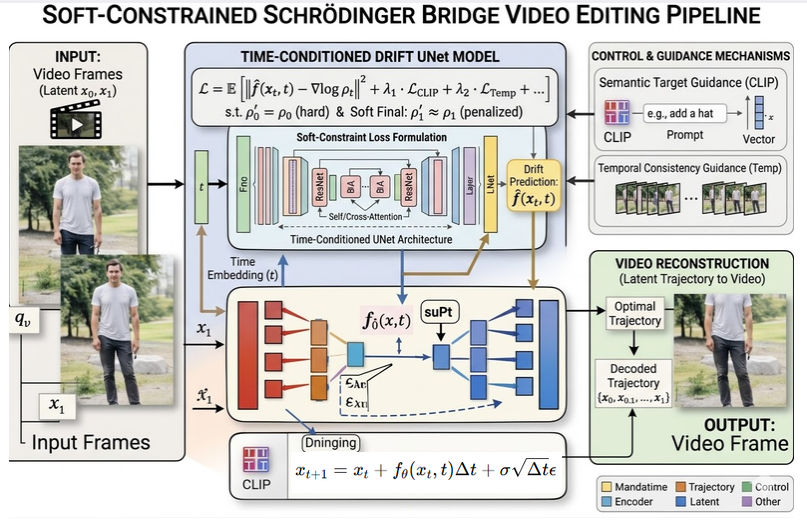
\includegraphics[width=\linewidth]{pipeline.png}
\caption{High-level soft-constrained Schr\"{o}dinger bridge video editing pipeline. The input video is encoded into Stable Diffusion VAE latents, edited through a prompt-conditioned bridge process with a frozen spatial U-Net and trainable temporal residual, and decoded back into output frames.}
\label{fig:pipeline}
\end{figure}

\subsection{Soft-Constrained Schr\"{o}dinger Bridge Objective}
Figure~\ref{fig:pipeline} summarizes the complete pipeline used in our implementation, from latent encoding and bridge-based drift learning to prompt-conditioned inference and VAE decoding.
Let $W$ denote a reference stochastic process (e.g., Brownian motion with drift), and let $\pi$ denote a candidate path measure over latent trajectories. A soft-constrained SB objective can be expressed as
\begin{equation}
\min_{\pi}\; \mathrm{KL}(\pi\,\|\,W) + \lambda\, \mathcal{D}(\pi_1,\rho_1),
\label{eq:sb_objective}
\end{equation}
where $\pi_1$ is the terminal marginal induced by $\pi$, $\rho_1$ is a desired target terminal distribution, $\mathcal{D}(\cdot,\cdot)$ is a divergence or discrepancy, and $\lambda$ controls the strength of the soft terminal constraint. In our setting, $\rho_1$ is induced by text guidance and optional temporal constraints.

In many practical settings, the constraint strength is scheduled over time to balance realism and semantic strength. We denote this as
\begin{equation}
\lambda = \lambda(t).
\label{eq:lambda_schedule}
\end{equation}

\subsection{Latent Video Representation}
Given an input video with frames $\{I_f\}_{f=1}^{F}$, we encode each frame using a pretrained Stable Diffusion VAE encoder $\mathcal{E}$:
\begin{equation}
\mathbf{x}_0 = \{x_{0,f}\}_{f=1}^{F},\quad x_{0,f} = s\,\mathcal{E}(I_f),
\end{equation}
where $x_{0,f}\in\mathbb{R}^{4\times H'\times W'}$ is the latent for frame $f$ and $s$ is the standard scaling factor used by Stable Diffusion. We decode edited latents using the VAE decoder $\mathcal{D}$.

\subsection{Stochastic Dynamics and Drift Parameterization}
We model latent evolution with an SDE
\begin{equation}
\mathrm{d}x_t = f_{\theta}(x_t,t, c)\,\mathrm{d}t + \sigma\,\mathrm{d}W_t,
\label{eq:sde}
\end{equation}
where $f_{\theta}$ is a time-conditioned drift network and $c$ is a conditioning signal derived from text (CLIP embeddings). In practice we use a simple interpolation corruption path that matches the repository implementation:
\begin{equation}
 x_t = (1-t)\,x_0 + t\,\epsilon + \sigma\sqrt{t(1-t)}\,z, \quad \epsilon,z\sim\mathcal{N}(0,I).
\label{eq:corruption_path}
\end{equation}

\subsection{DriftNet: Frozen Spatial Prior + Trainable Temporal Residual}
Our DriftNet combines a frozen Stable Diffusion 2D U-Net (per-frame spatial prior with cross-attention to text) and a lightweight 3D temporal residual head.

\paragraph{Variance scaling for compatibility with SD U-Net.}
For the interpolation in~\eqref{eq:corruption_path} (ignoring the $\sigma$ term), $\mathrm{Var}(x_t)$ scales as $(1-t)^2+t^2$. Stable Diffusion's U-Net is trained under a unit-variance assumption. We therefore rescale inputs as
\begin{equation}
\tilde{x}_t = \frac{x_t}{\sqrt{(1-t)^2+t^2 + \varepsilon}},
\label{eq:variance_scaling}
\end{equation}
matching the implementation.

\paragraph{From noise prediction to drift.}
The frozen SD U-Net predicts a noise residual $\hat{\epsilon}_\phi(\tilde{x}_t,t,c)$. For the linear path $x_t=(1-t)x_0+t\epsilon$, we can recover an estimate of $x_0$ via
\begin{equation}
\hat{x}_0 = \frac{x_t - t\,\hat{\epsilon}_\phi}{1-t+\varepsilon}.
\label{eq:x0_recovery}
\end{equation}
We then form a base drift estimate as
\begin{equation}
\hat{f}_{\text{base}}(x_t,t,c)=\hat{\epsilon}_\phi-\hat{x}_0.
\label{eq:base_drift}
\end{equation}

\paragraph{Temporal residual module.}
Let $\hat{f}_{\text{base}}\in\mathbb{R}^{F\times 4\times H'\times W'}$ denote the per-frame base drift. We apply a small 3D convolutional residual module $g_\psi$ across time and space:
\begin{equation}
\hat{f}_{\theta}=\hat{f}_{\text{base}} + g_{\psi}(\hat{f}_{\text{base}}),
\label{eq:temporal_residual}
\end{equation}
where only $\psi$ is trained. In the repository, $g_\psi$ consists of a $\text{Conv3D}(4\to32, k=(3,1,1))$ followed by SiLU and a $\text{Conv3D}(32\to4, k=(3,3,3))$ layer whose weights are zero-initialized to start from the pretrained spatial prior.

\subsection{Training Objective (Bridge Matching)}
We train the temporal residual parameters $\psi$ using a bridge matching loss. The repository uses a mean-squared error between predicted drift and an analytically constructed target drift:
\begin{equation}
\mathcal{L}_{\text{BM}} = \mathbb{E}_{t,\epsilon,z}\left[\left\|\hat{f}_{\theta}(x_t,t,c) - f^{\star}(x_t,t; x_0,\epsilon,z)\right\|_2^2\right].
\label{eq:bm_loss}
\end{equation}
For the simplified case $\sigma=0$, a common bridge-matching target is $f^{\star}\approx (x_1-x_0)$ with $x_1=\epsilon$. More generally, the implementation adds a volatility term with $\sigma>0$.

\subsection{Text Guidance and Soft Constraints}
Text prompts are encoded using CLIP to produce conditioning embeddings $c$. Soft constraints are incorporated as penalty terms that encourage semantic alignment at terminal time while avoiding brittle hard constraints:
\begin{equation}
\mathcal{L} = \mathcal{L}_{\text{BM}} + \lambda_\text{CLIP}\,\mathcal{L}_{\text{CLIP}} + \lambda_\text{Temp}\,\mathcal{L}_{\text{Temp}} + \cdots
\label{eq:full_loss}
\end{equation}
In this repository snapshot, conditioning is implemented by feeding text embeddings to the frozen SD U-Net cross-attention; the penalty-based extensions above are consistent with the provided project specification and can be added as additional losses.

\subsection{Inference via Backward Euler--Maruyama}
Given source latents $x_0$ and a starting noise level $t_\mathrm{start}\in(0,1]$, we initialize
\begin{equation}
 x \leftarrow (1-t_\mathrm{start})x_0 + t_\mathrm{start}\,\epsilon,
\end{equation}
and integrate backward using Euler--Maruyama for $K$ steps with step size $\Delta t=t_\mathrm{start}/K$:
\begin{equation}
 x \leftarrow x - \hat{f}_{\theta}(x,t,c)\,\Delta t + \eta\sqrt{\Delta t}\,\xi,\quad \xi\sim\mathcal{N}(0,I).
\label{eq:em}
\end{equation}
The repository omits the stochastic term in the final step to sharpen outputs. The final latent trajectory is decoded to frames using the Stable Diffusion VAE decoder.

\subsection{Algorithmic Summary}
We summarize the training and inference loops used in the reference implementation.

\paragraph{Training (temporal residual only).}
\begin{enumerate}
\item Sample a batch of cached video latents $x_0$ and corresponding text embeddings $c$.
\item Sample $t\sim\mathcal{U}(0,1)$ per sample and draw noise endpoints $\epsilon$.
\item Construct corrupted latents $x_t$ using~\eqref{eq:corruption_path}.
\item Predict drift $\hat{f}_\theta(x_t,t,c)$ using frozen 2D U-Net + temporal residual.
\item Minimize the bridge-matching loss in~\eqref{eq:bm_loss} with AdamW on temporal parameters.
\end{enumerate}

\paragraph{Inference (video-to-video editing).}
\begin{enumerate}
\item Load a source latent clip $x_0$ and encode a new prompt into conditioning $c$.
\item Initialize $x$ as a convex combination of $x_0$ and Gaussian noise at $t_\mathrm{start}$.
\item For $K$ steps, integrate backward using~\eqref{eq:em} with $t$ decreasing to $0$.
\item Decode the final latent trajectory with the VAE decoder to frames and write video.
\end{enumerate}

\section{Implementation Details}
The codebase provides a four-step pipeline aligned with Fig.~\ref{fig:pipeline}. We describe the implementation with emphasis on design choices that preserve compatibility with pretrained Stable Diffusion components.

\subsection{Data Source and Video Preprocessing}
Videos are downloaded from WebVid metadata, introduced with the Frozen-in-Time video--text retrieval dataset, using a multi-threaded downloader~\cite{bain2021frozen}. Each clip is decoded with OpenCV and resized to a fixed spatial resolution ($512\times512$ in the current configuration). For each video we extract up to $F=64$ frames; shorter videos are padded by repeating the last frame. Frames are normalized to $[-1,1]$ before VAE encoding.

\subsection{Latent and Text Cache}
To avoid repeatedly running large pretrained models during training, we cache (i) VAE latents and (ii) text embeddings on disk. Each frame is encoded using a Stable Diffusion VAE encoder and scaled by the Stable Diffusion latent scaling factor. Text is tokenized with the Stable Diffusion tokenizer and encoded by the Stable Diffusion text encoder. Latents are saved as tensors and later batched into $(B,F,4,H',W')$.

\subsection{Model Configuration}
DriftNet is implemented as a wrapper around a pretrained Stable Diffusion 2D U-Net. The 2D U-Net is frozen to preserve its spatial prior and reduce training compute. A lightweight temporal head (two 3D convolutions) is appended and trained as a residual correction. The last temporal layer is zero-initialized, ensuring that early in training the model reproduces the frozen 2D U-Net behavior and learns temporal corrections gradually.

\subsection{Training Protocol}
Training samples a random time $t\sim\mathcal{U}(0,1)$ for each video in the batch, constructs a corrupted latent $x_t$ using~\eqref{eq:corruption_path}, and minimizes an MSE bridge-matching objective between predicted drift and a target drift computed from endpoints and volatility. Only temporal parameters are optimized with AdamW, which decouples weight decay from adaptive gradient updates~\cite{loshchilov2019adamw}; the reference learning rate is $10^{-4}$. Checkpoints are written periodically.

\subsection{Inference Protocol (Video-to-Video Editing)}
The included inference script performs video-to-video editing rather than unconditional text-to-video generation. A source latent clip $x_0$ is loaded from the cache, mixed with Gaussian noise at a chosen start time $t_\mathrm{start}$ (default $0.8$), and integrated backward using Euler--Maruyama for $K=50$ steps. The final latent trajectory is decoded using the Stable Diffusion VAE decoder and written as an MP4.

\subsection{Hyperparameters and Defaults}
Table~\ref{tab:hyperparams} summarizes key defaults as implemented.

\begin{table}[t]
\caption{Reference hyperparameters from the repository implementation.}
\label{tab:hyperparams}
\centering
\begin{tabular}{@{}p{0.42\linewidth}p{0.48\linewidth}@{}}
\toprule
\textbf{Component} & \textbf{Setting} \\
\midrule
Video frames & $F=64$ (pad if shorter) \\
Frame size & $512\times512$ \\
Latent channels & $4$ (Stable Diffusion VAE) \\
Training epochs & $50$ \\
Batch size & $8$ (configurable) \\
Optimizer & AdamW (temporal layers only) \\
Learning rate & $10^{-4}$ \\
Bridge volatility & $\sigma=0.1$ (training corruption) \\
Inference steps & $K=50$ \\
Start time & $t_\mathrm{start}=0.8$ \\
\bottomrule
\end{tabular}
\end{table}

\subsection{Reproducibility Notes}
The code logs to a shared file and streams progress to console. For consistent runs, fixed random seeds, deterministic cuDNN settings (if desired), and version pinning for diffusers/transformers are recommended.

\paragraph{Summary of repository steps.}
For completeness, the pipeline can be executed in the following order: (i) download videos; (ii) extract and cache latents/text embeddings; (iii) train temporal layers; (iv) run inference for a new prompt.

\vspace{0.5em}
The codebase provides a four-step pipeline:
\begin{itemize}
\item \textbf{Video download:} fetch WebVid clips (up to a fixed cap) from metadata.
\item \textbf{Latent caching:} extract up to $F$ frames, resize, normalize, encode with Stable Diffusion VAE, and cache latents and text embeddings.
\item \textbf{Training:} freeze the Stable Diffusion U-Net; optimize only temporal layers with AdamW and MSE loss.
\item \textbf{Inference:} perform video-to-video editing by injecting noise into a cached latent clip and denoising under a new text prompt via backward Euler--Maruyama.
\end{itemize}

Unless otherwise specified, the reference implementation uses WebVid metadata, resizes frames to $512\times512$, caches up to $F=64$ frames, trains for $50$ epochs with AdamW at learning rate $10^{-4}$ (temporal layers only), and performs inference for $K=50$ solver steps starting from $t_\mathrm{start}=0.8$.

\section{Experimental Setup}
This repository snapshot is a proof-of-concept implementation. It includes training and inference code but does not yet ship an evaluation harness with automated metrics.

\subsection{Tasks}
We consider text-guided video-to-video editing: given a source clip, edit semantic attributes (e.g., appearance, style) while maintaining motion and scene structure. The reference inference script explicitly follows this setting by starting from a partially noised version of a real source latent and denoising under the edited prompt.

\subsection{Baselines}
Suitable baselines include (i) per-frame latent diffusion editing with identical prompt (no temporal head), (ii) temporal smoothing post-processing on per-frame outputs, and (iii) existing video diffusion/editing models when available. In this repository, a natural internal baseline is to disable the temporal residual block and use only the frozen 2D U-Net drift.

\subsection{Metrics}
This snapshot reports quantitative evaluation using semantic alignment, perceptual similarity, reconstruction fidelity, and temporal consistency metrics. CLIP Score and CLIPSIM measure text--video semantic alignment using the CLIP embedding space~\cite{radford2021clip}. LPIPS measures learned perceptual distance~\cite{zhang2018lpips}, SSIM and PSNR measure frame-level fidelity with SSIM emphasizing structural similarity~\cite{wang2004ssim}, and warp error measures temporal consistency using optical-flow-based alignment, commonly estimated with methods such as RAFT~\cite{teed2020raft}.

\section{Results}
The repository used an AMD MI300X GPU for training on a small WebVid subset. We additionally include training, inference, and quantitative evaluation observations from the recorded runs.

\subsection{Training Dynamics}
The temporal residual was trained on 472 videos for 40 epochs using an AMD MI300X GPU with a limited training budget. The bridge-matching loss fluctuated between 0.7595 (epoch 20) and 1.2675 (epoch 35). Because the target drift is constructed from randomized noise endpoints (the $\epsilon$ term in the corruption path), the loss is not expected to converge to zero. Table~\ref{tab:train_loss} lists representative checkpoints.

\begin{table}[t]
\caption{Training loss (bridge-matching MSE) at selected epochs.}
\label{tab:train_loss}
\centering
\begin{tabular}{@{}p{0.20\linewidth}p{0.28\linewidth}@{}}
\toprule
\textbf{Epoch} & \textbf{Avg. Loss} \\
\midrule
1 & 0.8271 \\
10 & 1.1406 \\
20 & 0.7595 \\
30 & 1.0927 \\
40 & 0.7763 \\
\bottomrule
\end{tabular}
\end{table}

As shown in Table~\ref{tab:train_loss}, the training loss does not decrease monotonically across epochs. The loss starts at 0.8271 in epoch 1, rises to 1.1406 by epoch 10, reaches its lowest listed value of 0.7595 at epoch 20, increases again at epoch 30, and finishes at 0.7763 in epoch 40. This behavior is consistent with the stochastic bridge formulation: each training step samples noisy intermediate states and randomized target endpoints, so the objective measures how well the drift field matches a changing denoising direction rather than a fixed deterministic target. The final epoch returning close to the best observed loss suggests that the temporal residual learns a usable drift estimate within the limited AMD MI300X training run, even though the fluctuations indicate that the model has not fully stabilized.

\subsection{Evaluation Results}
Table~\ref{tab:eval_metrics} summarizes the evaluation results. The model achieved a CLIP Score of 0.2213 and CLIPSIM of 0.8799, indicating that the edited videos retain meaningful alignment with the input prompts. The reconstruction-oriented metrics show moderate source preservation, with SSIM of 0.5946 and PSNR of 19.7504 dB. LPIPS of 0.5618 reflects visible perceptual changes from the source videos, while the warp error of 500.5221 indicates that temporal consistency remains a major area for improvement.

\begin{table}[t]
\caption{Evaluation metrics over generated videos.}
\label{tab:eval_metrics}
\centering
\footnotesize
\begin{tabular}{@{}p{0.24\linewidth}p{0.14\linewidth}p{0.14\linewidth}p{0.22\linewidth}@{}}
\toprule
\textbf{Metric} & \textbf{Mean} & \textbf{Std.} & \textbf{Direction} \\
\midrule
CLIP Score & 0.2213 & 0.0272 & Higher is better \\
CLIPSIM & 0.8799 & 0.0293 & Higher is better \\
LPIPS & 0.5618 & 0.1344 & Lower is better \\
SSIM & 0.5946 & 0.1376 & Higher is better \\
PSNR (dB) & 19.7504 & 2.8301 & Higher is better \\
Warp Error & 500.5221 & 292.2662 & Lower is better \\
\bottomrule
\end{tabular}
\end{table}

The metrics in Table~\ref{tab:eval_metrics} show the expected tradeoff for prompt-guided video editing. The high CLIPSIM value indicates that the generated clips are semantically close to the text conditioning, while the lower CLIP Score suggests that prompt alignment can still be strengthened. The SSIM and PSNR values indicate that the edited outputs preserve part of the source structure, but not as a near-identical reconstruction; this is desirable for editing, where some visual change is required. At the same time, the LPIPS value and large warp error show that perceptual deviation and temporal instability remain visible. Overall, the obtained results indicate that the model can produce prompt-aligned edits after 40 epochs, but stronger temporal regularization or longer training would be needed to reduce frame-to-frame artifacts.




\section{Discussion and Limitations}
Freezing the pretrained spatial U-Net reduces training cost but also limits the capacity for large structural edits. The epoch-wise behavior in Table~\ref{tab:train_loss} suggests that the lightweight temporal residual can learn a useful bridge drift under a constrained training budget, but the non-monotonic loss curve also shows that the optimization remains noisy. The quantitative results in Table~\ref{tab:eval_metrics} further support this interpretation: semantic alignment is reasonable, but temporal consistency and perceptual smoothness are not yet strong enough for high-fidelity video editing. The current implementation relies on cached WebVid latents and a simplified SB corruption path, and it does not yet include explicit CLIP loss backpropagation through sampling. Future work can incorporate adaptive $\lambda(t)$ schedules, explicit terminal penalties $\mathcal{D}(\pi_1,\rho_1)$, and stronger temporal objectives.

\subsection{Scope of Edits}
The repository demonstrates prompt-conditioned video-to-video editing by starting from a noised source trajectory. This setting is well-suited to attribute/style changes that preserve global structure. More aggressive edits (changing layout, geometry, or long-term identity) may require training additional parameters beyond the temporal residual head or incorporating stronger conditioning and constraints.

\subsection{Evaluation Gaps}
The current evaluation is limited to the recorded WebVid subset and does not yet include comparisons against external video-editing baselines. Future evaluation should add benchmark splits, human preference studies, and ablations over the temporal residual module and solver settings.

\subsection{Guidance as Constraints vs. Conditioning}
In the present snapshot, text guidance is applied through conditioning (cross-attention) in the frozen Stable Diffusion U-Net. The project motivation additionally describes CLIP-based soft constraints as penalty terms; implementing these penalties requires differentiable evaluation of semantic similarity along the trajectory and careful scheduling of $\lambda(t)$.

\section{Conclusion}
We described a soft-constrained Schr\"{o}dinger bridge formulation for text-guided video editing in latent space. By leveraging a frozen Stable Diffusion prior for spatial structure and training only a lightweight temporal residual drift head, the approach aims to preserve realism while improving temporal coherence under text-driven edits. Backward Euler--Maruyama sampling in VAE latents enables an efficient video-to-video editing workflow.

\section*{Acknowledgment}
We express our sincere gratitude for providing us the opportunity to undertake this project as part of the Mathematical Modelling course. This project enabled us to apply theoretical concepts to a practical, real-world problem and strengthened our understanding of mathematical and machine learning concepts

\bibliographystyle{IEEEtran}
\bibliography{refs}

\end{document}
